% Cover page - packages already loaded in main document
% Additional tikz library for backgrounds
\usetikzlibrary{backgrounds}
% Declare the pgf layers
\pgfdeclarelayer{background}
\pgfdeclarelayer{foreground}
\pgfsetlayers{background,main,foreground}

% Definición de colores específicos para portada
\definecolor{verdeSuave}{HTML}{90EE90}
% Note: RCimat and GCimat colors are redefined here with different values
% than in Preambulo.tex - consider using consistent colors
\definecolor{RCimatPortada}{HTML}{00796B} 
\definecolor{GCimatPortada}{HTML}{388E3C}

\begin{titlepage}

% Fondo con TikZ
\tikz[remember picture,overlay] \node[opacity=1.0, inner sep=0pt] at ([yshift=-2.5cm]current page.south){

\begin{tikzpicture}
    \begin{pgfonlayer}{background}
        \filldraw[RCimatPortada] (-12,-8)--(-12,3)--(12,2)--(12,-8)--cycle;
    \end{pgfonlayer}

    \begin{pgfonlayer}{foreground}
        \filldraw[GCimatPortada] (-12,0)--(-12,1)--(12,1)--(12,0)--cycle;
    \end{pgfonlayer}
\end{tikzpicture}};

% Título
\par\noindent
{\bfseries\Huge  Cómputo Estadístico | Tarea \#2}
\vspace{0.2cm}

\par\noindent
\LARGE Aplicaciones de Modelos Lineales Generalizados\\
\rule[0.3cm]{\linewidth}{2pt}

% Integrante
\vspace{0.5cm}
\begin{minipage}{0.6\textwidth}
    \begin{flushleft} \large
        {\emph{\textbf{César M. Aguirre Calzadilla}}}\\
    \end{flushleft}
\end{minipage}

% Logo y datos institucionales
\vspace{0.1cm}
\begin{center}
    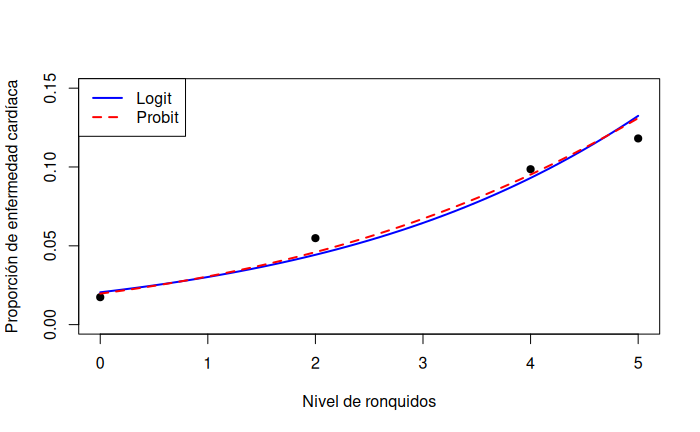
\includegraphics[scale=0.6]{Images/logit-probit-p02.png}\par
    \vspace{1cm}
    {\textit{\bfseries\huge Centro de Investigación en Matemáticas}\par}
    \vspace{0.5cm}
    {\large Maestría en Cómputo Estadístico\par}
    % {\large Ciencia de Datos\par} % opcional
    \vspace{1cm}
\end{center}

% Profesores y fecha
\begin{center} \large
    {\emph{\textbf{Catedráticos:}}}\\
    \large ME. José Ramón Domínguez Molina\par
    \large Dr. Rodrigo Macías Paéz\par
    \vspace{0.3cm}
    \large \today
\end{center}

\end{titlepage}

